\chapter{Authentication techniques protocols, and architectures}

Authentication refers to the process of verifying the identity of an entity (whether it's a human, software component, or hardware element) 
before granting access to resources in a system. Authentication can be applied to various type of "actors", such as:
\begin{itemize}
    \item \textbf{Human being}
    \item \textbf{Software component}
    \item \textbf{Hardware element}
\end{itemize}

\subsubsection{Authentication vs Authorization}
\begin{itemize}
    \item \textbf{Authentication (authC/authN)}: established the identity of an entity.
    \item \textbf{Authorization (authZ)}: determines where a authenticated entity has permission to access.
\end{itemize}

\section{Authentication factors}
Authentication can be based on 3 primary factors:
\begin{itemize}
    \item \textbf{Knowledge}: Information that only the user knows and can provides as proof of their identity.
    \item \textbf{Ownership}: Physical object or device that only the user has access to.
    \item \textbf{Inherence}: This factor relies on unique biological traits of the user (e.g fingerprint).
\end{itemize}
\textcolor{red}{N.B} Authentication can be applied not just to human user, but also to processes and devices.

\subsection{Risks}
\begin{itemize}
    \item \textbf{Knowledge:}
    \begin{itemize}
        \item \underline{Storage} \(\rightarrow \) if passwords are stored improperly, they are vulnerable to thefts. 
        \item \underline{Demonstration} \(\rightarrow\) user might inadvertently reveal their password through social engineering.
        \item \underline{Transmission} \(\rightarrow\) if passwords are sent over insecure channel, they can be intercepted by attackers. 
    \end{itemize}
    \item \textbf{Ownership:}
    \begin{itemize}
        \item \underline{Authentication thieft}
        \item \underline{Cloning}
        \item \underline{Unathorized usage}
    \end{itemize}
    \item \textbf{Inherence:}
    \begin{itemize}
        \item \underline{Counterfeiting} \(\rightarrow\) biometric data can be spoofed or replicated by attackers using sophisticated techniques.
        \item \underline{Privacy} \(\rightarrow\) the use of biometric data raises the risk of biometric information being exposed.
        \item \underline{Irreversibility} \(\rightarrow\) biometric traits cannot be replaced if compromised. 
    \end{itemize}
\end{itemize}

\section{Digital Authentication model (NIST SP800.63B)}
\begin{figure}[H]
    \centering
    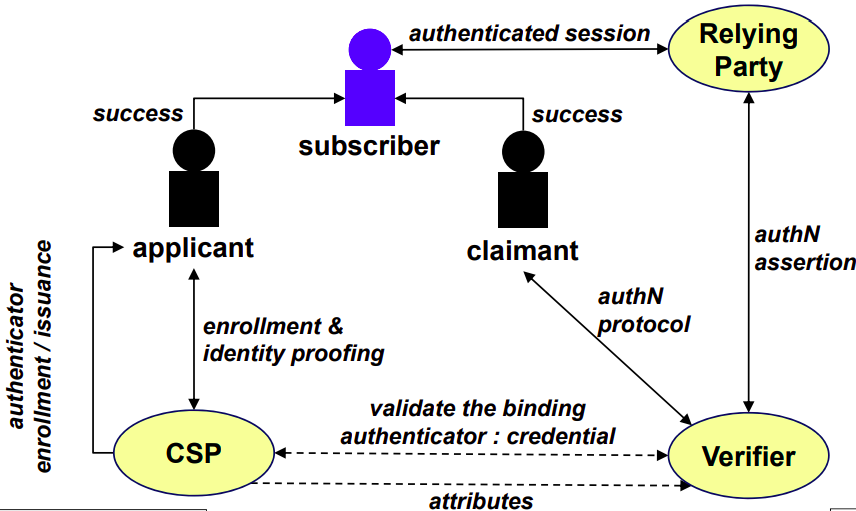
\includegraphics[width=0.5\textwidth]{/home/lorenzo/Notes/Information System Security/images/Screenshot from 2024-11-13 20-29-06.png}
\end{figure}
\textbf{Entities:}
\begin{itemize}
    \item \textbf{Subscriber}: applicant who has successfully completed identity proofing.
    \item \textbf{Applicant}: an individual applying to established a digital identity.
    \item \textbf{Claimant}: the user trying to prove their identity to access a system or service.
    \item \textbf{Relying Party}: entity (e.g service provider, website) that requests/receives an authN assertion from the verifier to asses user identity (and attributes).
    \item \textbf{Verifier}: validates the user's credential during each authentication event. 
    \item \textbf{CSP}: an entity that issues, manages, and maintains \textbf{credentials} used by individuals to authenticate themselves. 
\end{itemize}
\begin{quotebox-red}{Applicant vs Claimer}
    An applicant needs to enroll in the system for the first time to establish their identity. Instead, a claimant asserts their identity to gain access to the system after enrollment.
\end{quotebox-red}


\section{Generic authentication protocol}
\begin{minipage}{0.5\textwidth}
    \begin{enumerate}
        \item The user initiates an authentication request by sending their UID.
        \item The user generates a proof based on their secret, using a secure function \(F(S_{UID})\), and send this proof to the verifier.
        \item The verifier checks if the received proof matches the stored representation of the secret.
        \item If it matches, the user is successfully authenticated.
    \end{enumerate}
\end{minipage} 
\hspace{1cm}
\begin{minipage}{0.5\textwidth}
    \centering
    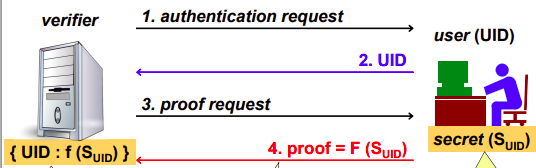
\includegraphics[width=\textwidth]{/home/lorenzo/Notes/Information System Security/images/Screenshot from 2024-11-14 11-06-55.png}
\end{minipage}



\section{Password base authentication}
\begin{minipage}{0.5\textwidth}
    \begin{enumerate}
        \item The user sends their UID and \(P_{UID}\) (= Password) to the verifier.
        \item The server verifies the proof:
        \begin{itemize}
            \item If password are stored in cleartext, it directly compares the proof with the stored password.
            \item If password are stored in hashes, it hashes the proof and compares it to the store hash \(H_{UID}\).
        \end{itemize}
    \end{enumerate}
\end{minipage} 
\hspace{1cm}
\begin{minipage}{0.5\textwidth}
    \centering
    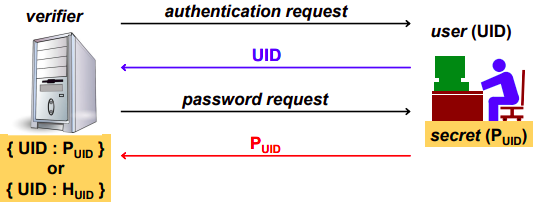
\includegraphics[width=\textwidth]{/home/lorenzo/Notes/Information System Security/images/Screenshot from 2024-11-14 11-09-10.png}
\end{minipage}

\begin{quotebox-yellow}{Problems of reusable Passowrds}
    \begin{itemize}
        \item \textbf{PWD Sniffing} (attackers intercept password during transmission)
        \item \textbf{PWD Database attack} (if DB contains plaintext or obfuscated PWD)
        \item \textbf{PWD Guessing} (very dangerous if it can be done offline, e.g against a list of PWD hashes)
        \item \textbf{PWD Enumeration} (PWD brute force attack)
        \begin{itemize}
            \item If PWD is limited in length and/or character type.
            \item If authN protocol does not block repeated failures.
        \end{itemize}
        \item \textbf{PWD Duplications} (using the same PWD for one service against another one, due to user PWD reuse)
        \item \textbf{Cryptographic Aging} (as computing power grows, older cryptographic methods become vulnerable to new attacks)
        \item \textbf{PWD capture via server spoofing and phishing} (attackers deceive user into giving away their PWD by pretending to be legitimate service)
    \end{itemize} 
\end{quotebox-yellow}



\begin{quotebox-grey}{Password best practies}
    Suggestion to reduce password risks:
    \begin{itemize}
        \item Use alphabetical characters (upper case + lower case), digits and special characters
        \item Make passwords long (at least 8 character)
        \item Never use dictionary words
        \item Change password regularly, but not too frequently
        \item Do not reuse passwords across different services
    \end{itemize}
\end{quotebox-grey}


\begin{quotebox-yellow}{Password storage}
    \begin{itemize}
        \item \textbf{Server Side:}
        \begin{itemize}
            \item Passwords should never be stored in cleartext.
            \item \underline{Encrypted passwords} aren't ideal since the server would need to know the encryption key.
            \item \underline{Better to store a password digest} (hashed password), though vulnerable to dictionary attacks.
            \item \underline{Rainbow tables} can speed up these attacks, so it’s important to add a “salt” (random variation) to each password.
        \end{itemize}
        \item \textbf{Client-side:}
        \begin{itemize}
            \item Ideally, passwords are memorized by the user, but having many passwords makes this difficult.
            \item People may resort to writing them down or using simple passwords, which is risky.
            \item \underline{Using a password manager} or encrypted file is a safer alternative.
        \end{itemize}
    \end{itemize}
\end{quotebox-yellow}


\section{The "dictionary" attack}
\begin{itemize}
    \item \textbf{Hypothesis:} The attacker knows the hash algorithm and the hashed password values.
    \item \textbf{Pre-computation:} For each word in a dictionary, compute and store its hash \(store(DB,Word,hash(World))\)
    \item \textbf{Attack process:}
    \begin{itemize}
        \item Let \(HP\) (=hash password) to be the hash of an unknown password.
        \item Lookup \(HP\) in the precomputed dictionary \((DB)\) to find a matching password.
        \item If found, output the password; if not, indicate it's "not in dictionary".
    \end{itemize}
\end{itemize}

\section{Rainbow Table attack}
Rainbow Table is a \textbf{space-time trade-off technique} that reduces storage needs for exhaustive hash tables, making certain brute-force attacks feasible within limited space.
It uses a reduction function \(r:h \rightarrow p\) (which is NOT \(h^{-1}\)) to generate chains of hashes.
\\ \textbf{Example:}
\begin{itemize}
    \item For a 12-digit password, an exhaustive hash table would require \(10^{12}rows(P_i:HP_i)\) 
    \item rainbow = \(10^9\) rows, each representing 1000 possible passwords.
\end{itemize}

\begin{center}
\begin{minipage}{0.5\textwidth}
    \begin{quotebox-red}{Attack}
        \centering
        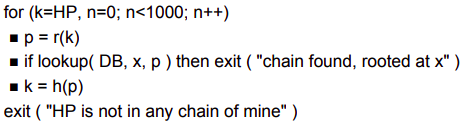
\includegraphics[width=0.8\textwidth]{/home/lorenzo/Notes/Information System Security/images/Screenshot from 2024-11-14 11-51-24.png}
\end{quotebox-red}
\end{minipage}
\end{center}

\section{Salting Passwords: A Defense Against Dictionary and Rainbow Table Attacks}
\textbf{Salting passwords} is a security technique used to protect stored passwords from dictionary attacks and rainbow table attacks. A salt is a unique, random string added to each password before hashing. This ensures that even if two users have the same password, their hashes will be different due to the unique salt.
\newline
\newline
\begin{minipage}[t]{0.5\textwidth}
    \subsubsection{Steps for each user (UID):}
    \begin{itemize}
        \item Generate or ask for the user's password.
        \item Create a unique, random slat for each user.
        \item Compute the salted hash: \(SHP=hash(password\ ||\ salt)\)
        \item Store the triplet \(\{UID,\ SHP,\ salt\}\)
    \end{itemize}
\end{minipage} 
\hspace{0.5cm}
\begin{minipage}[t]{0.5\textwidth}
    \subsubsection{Password Verification with Salt}
   \begin{itemize}
    \item \textbf{Claimant:} Provides their user ID (UID) and password (PWD).
    \item \textbf{Verifier:} 
    \begin{itemize}
        \item Uses the UID to find the stored salted hash (SHP) and salt. 
        \item Computes \(SHP'=hash(PWD\ || \ salt)\).
    \end{itemize}
   \end{itemize}
\end{minipage}

\begin{quotebox-yellow}{The Linkedin attack}
    In 2012, LinkedIn was breached, exposing 6.5 million unsalted SHA-1 password hashes. The lack of salting allowed attackers to crack at least 236,578 passwords through crowdsources efforts before restrictions halted the exposure.
\end{quotebox-yellow}

\noindent{\color{gray!50}\rule{\textwidth}{0.5pt}}


\section{Strong authentication definitions}
The concept of strong authentication (authN) is crucial in ensuring secure identity verification, but it has never been formally defined with a universal definition.
Various definitions exist depending on the context, such as the European Central Bank (ECB) and PCI-DSS.

\begin{quotebox}[colframe=blue!10!white, colback=blue!5!white]{ECB definition}
    The ECB defines strong authentication as a process that involves at least two independent 
    elements from \textbf{knowledge} (e.g. password), \textbf{ownership} (e.g. smartcard), 
    and \textbf{inherence} (e.g. biometrics). The key requirement is that these elements 
    must be mutually independent, so compromising one should not affect the others. 
    Furthermore, at least one element should be \textbf{non-reusable} or \textbf{non-replicable} 
    (except for inherence), with the entire process safeguarding the confidentiality of the 
    authentication data.
\end{quotebox}

\begin{quotebox}[colframe=blue!10!white, colback=blue!5!white]{PCI-DSS Definition}
    PCI-DSS mandates \textbf{multi-factor authentication (MFA)} for access to cardholder data, 
    particularly for administrators and remote access from untrusted networks. Since version 3.2, MFA has become compulsory for remote access, 
    and the use of the same factor twice (e.g., two passwords) does not qualify as MFA.
\end{quotebox}

\section{Challenge-Response Authentication (CRA)}
Challenge-response authentication (CRA) is a widely used technique where 
a challenge is issued, and the claimant responds by solving it with a 
secret (shared or private). The challenge must be \textbf{non-repeatable} 
(usually a random nonce) to avoid replay attacks. The function used to compute 
the response must be \textbf{non-invertible}, otherwise, a listener can record the 
traffic and easily find the shared secret:
\[ if(\exists f^{-1})\ then\ K_c\ =\ f^{-1}(response, challenge)\]

\subsection{Symmetric CRA}
\begin{minipage}{0.3\textwidth}
    \vspace{-0.9cm}
    In symmetric CRA, both the client and the server share a secret key that is used to verify the authenticity of a user or system This method is fast, often utilizing hash 
    functions (e.g., SHA1, SHA2, SHA3).
\end{minipage} 
\hspace{0.001cm}
\begin{minipage}{0.7\textwidth}
    \centering
    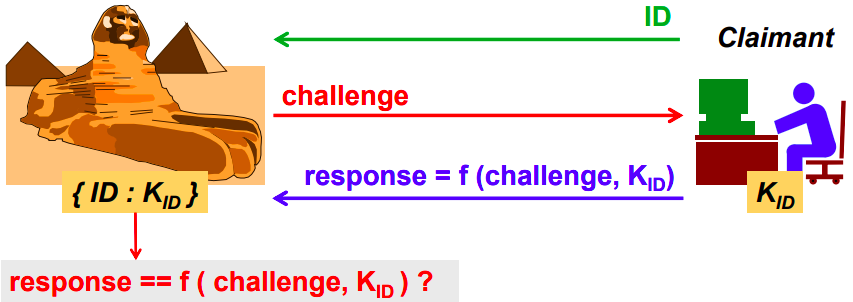
\includegraphics[width=0.7\textwidth]{/home/lorenzo/Notes/Information System Security/images/Screenshot from 2024-11-14 18-31-56.png}
\end{minipage}

\subsection{Mutual symmetric CRA}
Mutual symmetric CRA requires both parties to authenticate each other.
However, it's a old protocols so it has many vulnerabilities.

\subsubsection{Version 1: Basic Exchange}
\begin{minipage}{0.5\textwidth}
In this case, the initiator explicitly provides its claimed identity (This version is considered outdated and insecure).
\\\textbf{Process:} 
\begin{itemize}
    \item Alice sends an encrypted challenge (\(C_B\)) to Bob using the shared key \(K_{AB}\).
    \item Bob responds with an encrypted challenge (\(C_A\)) for Alice, also using \(K_{AB}\).
\end{itemize}
\end{minipage} 
\hspace{0cm}
\begin{minipage}{0.5\textwidth}
    \centering
    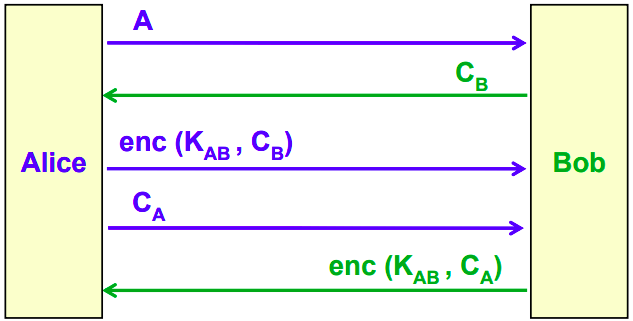
\includegraphics[width=0.7\textwidth]{/home/lorenzo/Notes/Information System Security/images/Screenshot from 2024-11-15 11-52-51.png}
\end{minipage}

\subsubsection{Version 2: Improved Performance}
\begin{minipage}{0.5\textwidth}
    Optimized by reducing the number of messages, which improves performance without compromising security.
    \\ \textbf{Process:}
    \begin{itemize}
        \item Alice includes her identity \((C_A)\) and sends an encrypted challenge (\(C_B)\) in the same message.
        \item Bob responds with his encrypted challenge \(C_A\) to complete the exchange.
    \end{itemize} 

\end{minipage} 
\hspace{0cm}
\begin{minipage}{0.5\textwidth}
    \centering
    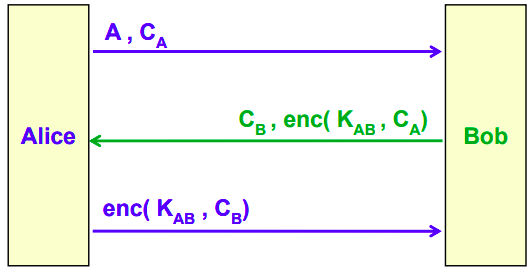
\includegraphics[width=0.7\textwidth]{/home/lorenzo/Notes/Information System Security/images/Screenshot from 2024-11-15 12-04-56.png}
\end{minipage}

%Now I give you some text and I want that you resume it. I don't want many list (this it no means that I don't want there to be any) I want also that you reorganized the sections 
\begin{quotebox}[colframe=blue!10!white, colback=blue!5!white]{Attack on Mutual Symmetric CRA}
    \begin{minipage}{0.5\textwidth}
        \vspace{-0.5cm}
        A potential attacker, "Mike" (posing as Alice), exploits the protocol by mimicking responses:
        \begin{itemize}
            \item The attacker intercepts Alice's identity \((C_A)\) and Bob's challenge \((C_B)\).
            \item The attacker uses the shared key \(K_{AB}\) to manipulate responses and mimic both parties.
        \end{itemize}
    \end{minipage} 
    \hspace{1cm}
    \begin{minipage}{0.3\textwidth}
        \centering
        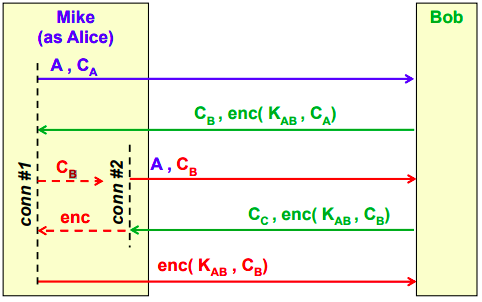
\includegraphics[width=\textwidth]{/home/lorenzo/Notes/Information System Security/images/Screenshot from 2024-11-15 12-09-09.png}
    \end{minipage}
\end{quotebox}

\subsection{Asymmetric CRA}
\begin{minipage}{0.6\textwidth}
%	\vspace{-0.5cm}
    \textbf{Process:}
    \begin{itemize}
        \item A \textbf{random nonce (R)} is generated by the Verifier.
        \item The verifier encrypts \(R\) using the user's public key (\(ID.PK\)) and sends it to the Claimant:
        \(C=enc(ID.PK,R)\)
        \item The Claimant decrypts \(C\) using their private key (\(ID.SK\)) and sends \(R\) back in cleartext:
        \(response=dec(ID.SK,C)\)
        \item The Verifier validates: \(valid(ID)\ \&\&\ (response\ ==\ R)\).
    \end{itemize}
\end{minipage} 
\hspace{0.2cm}
\begin{minipage}{0.4\textwidth}
    \centering
    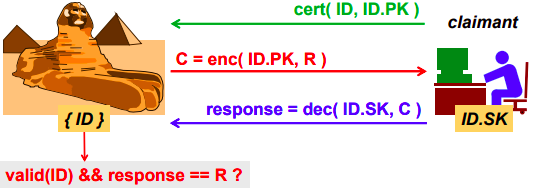
\includegraphics[width=\textwidth]{/home/lorenzo/Notes/Information System Security/images/Screenshot from 2024-11-15 12-43-33.png}
\end{minipage}
\subsubsection{Applications}
\begin{itemize}
    \item  Widely implemented in secure communication protocols like IPsec, SSH, and TLS.
    \item Fundamental in modern authentication frameworks such as FIDO.
\end{itemize}
\begin{quotebox}[colframe=blue!10!white, colback=blue!5!white]{Asymmetric CRA analysis}
    \begin{minipage}{0.5\textwidth}
        \vspace{-1.1cm}
        \subsubsection{Security:}
        \begin{itemize}
            \item It's the strongest mechanism.
            \item Does not require the Verifier to store any shared secret, reducing potential attack vectors.
        \end{itemize}
     \end{minipage} 
     \hspace{0cm}
     \begin{minipage}{0.5\textwidth}
        \subsubsection{Problems:}
        \begin{itemize}
            \item It \textbf{slower} compared to symmetric methods.
            \item If designed inaccurately may lead to an involuntary signature
            by the Claimant.
            \item Trust issues managing root certificates, name constraint, and certificate revocation.
        \end{itemize}
     \end{minipage}
\end{quotebox}

\section{One-Time Password(OTP)}
\begin{minipage}{0.6\textwidth}
\vspace{-1.0cm}
One-Time Passwords are temporary and valid for a single use in an authentication session. They mitigate risks like password reuse and passive sniffing but can still be vulnerable to man-in-the-middle (MITM) attacks. These passwords are often designed  with random characters to prevent guessing, but this can make password insertion difficult for users. 
\end{minipage} 
\hspace{0.5cm}
\begin{minipage}{0.4\textwidth}
    
    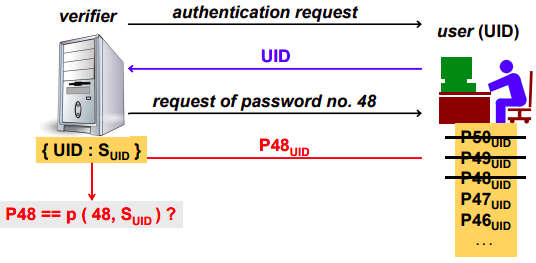
\includegraphics[width=0.8\textwidth]{/home/lorenzo/Notes/Information System Security/images/Screenshot from 2024-11-15 13-11-17.png}
\end{minipage}

\subsection{S/KEY System}
S/KEY System was the first OTP implementation by Bell Labs (1981).
It pre-computes a sequence of passwords derived from a user’s secret. 
Each password is validated and replaced with its predecessor, ensuring security 
without storing the secret:
\[Secret = S_{ID}\]
\[P_1=h(S_{ID}),P_2=h(P_1),...,P_N=h(P_{N-1})\]
\noindent
This approach minimizes verifier storage needs and offers robust protection, with users solely responsible for password retention.\\
\begin{customquote}
    \textbf{One-time generation with S/KEY}
    \\In the S/KEY system, the user creates 
    a secret passphrase (PP), which is combined 
    with a server-provided seed to generate a 64-bit 
    password. The passphrase is concatenated with the seed, 
    and an MD4 hash is used to produce the password. 
    The result is presented as six short words from a shared 
    dictionary, making it easy to remember. This method allows secure password generation while using the same passphrase across multiple servers with different seeds. If the passphrase is compromised, security is at risk.
\end{customquote}



\subsection{Time-based OTP (TOPT)}
\begin{minipage}{0.5\textwidth}
    TOTP systems generate passwords based on the user's secret and the current time, requiring synchronization between the user and the verifier:
    \[p(ID,t)\ =\ h(t,S_{ID})\]
    \begin{customquote}
        \textbf{Authentication Process:}
        \begin{itemize}
            \item The claimant sends an authentication request with \(ID\) and the generated OTP \(x\).
            \item The verifier checks if \(X\) matches the computed OTP for the corresponding \(ID\) and \(t\).
        \end{itemize}
    \end{customquote}
    
\end{minipage} 
\hspace{0.3cm}
\begin{minipage}{0.5\textwidth}
    \centering
    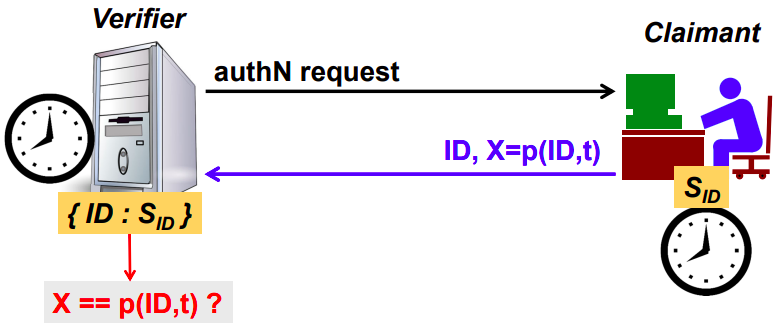
\includegraphics[width=0.9\textwidth]{/home/lorenzo/Notes/Information System Security/images/Screenshot from 2024-11-16 10-54-11.png}
\end{minipage}

\vspace{0.5cm}
\begin{customquote}
    \textbf{Requirements:}
    \begin{itemize}
        \item Local computation of OTPby the subscriber.
        \item Clock synchronization  (or keeping track of time-shift for each subscribers).
    \end{itemize}
\end{customquote}

\begin{customquote}
    \textbf{Limitations:}
    \begin{itemize}
        \item Only one authentication is allowed per time-slot, typically 30s or 60s.
        \item This time limit may not suit all services.
    \end{itemize}
\end{customquote}

\begin{customquote}
    \textbf{Vulnerabilities:}
    \begin{itemize}
        \item Potential attacks on the subscriber and verifier:
        \begin{itemize}
            \item Fake NTP servers or compromised mobile network femtocells.
            \item Sensitive database storage at the verifier (e.g., the RSA SecurID attack).
        \end{itemize}
    \end{itemize}
\end{customquote}

\begin{quotebox}[colframe=blue!10!white, colback=blue!5!white]{Example: RSA SecurID}
    \begin{minipage}{0.6\textwidth}
    %	\vspace{-0.5cm}
        Authentication process:
        \begin{itemize}
            \item \textbf{The claimant sends to the verifier:}
            \begin{itemize}
                \item \underline{Without PIN Pad:} User ID, PIN, and Token Code (computed using seed and time).
                \item \underline{With PIN Pad:} User ID and a combined Token Code* (includes seed, time, and PIN).
            \end{itemize}
        \end{itemize}
    \end{minipage} 
    \hspace{1cm}
    \begin{minipage}{0.3\textwidth}
        \centering
        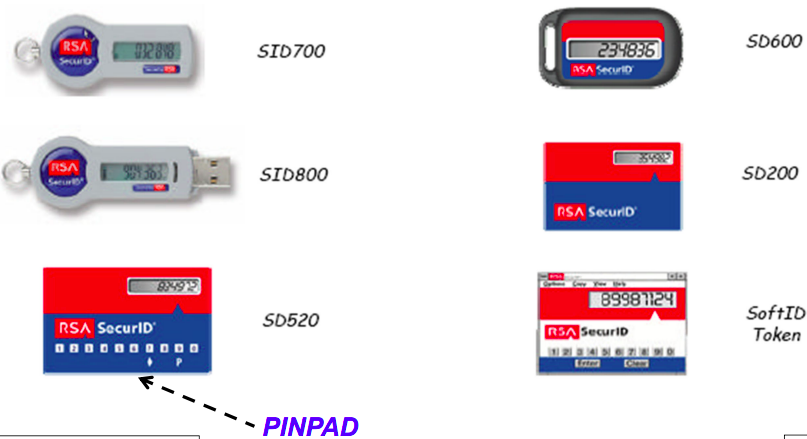
\includegraphics[width=1.1\textwidth]{/home/lorenzo/Notes/Information System Security/images/Screenshot from 2024-11-16 12-00-37.png}
    \end{minipage}
\end{quotebox}

\subsection{Out-of-Band (OOB) OTP}
Out-of-Band OTP requires a \textbf{secure channel} with server authentication 
to prevent MITM (Man-In-The-Middle) attacks. Traditionally, it uses text or 
SMS as the communication channel, but this method is increasingly vulnerable 
due to weaknesses in VoIP, mobile user identification, and the SS7 protocol. 
Nowadays, a push mechanism over a \textbf{TLS-secured channel} to a registered device is recommended for enhanced security.


\subsection{Two-/Multi-Factor Authentication (2FA/MFA)}
MFA enhances authentication (authN) by requiring multiple factors, 
such as a PIN, OTP, or biometrics, to verify identity. These factors can include something you know (like a PIN or password), something you have (like a token or phone), and something you are (like biometric data). MFA also protects the authenticator, for example, by using a PIN to safeguard it, but risks arise if the lock mechanism is weak or if there’s no protection against multiple unlock attempts.

\begin{quotebox-grey}{Importance of MFA: The iPhone Ransomware (2014)}
    In 2014, iCloud accounts with 1FA were hacked, allowing attackers to lock devices remotely. Victims were extorted for \$100, but paying didn’t help as the PayPal account was fake. This incident underscores the need for MFA to secure devices and prevent such attacks.
\end{quotebox-grey}

\section{Authentication of human beings}
To verify whether we're interacting with a human rather than a machine, there are two common approaches:
\begin{itemize}
    \item \textbf{CAPTCHA (Completely Automated Public Turing Test to Tell Computers and Humans Apart):} A method where users must solve challenges like distorted characters in images to prove they are human.
    \item \textbf{Biometric Techniques:} 
    These involve verifying human characteristics such as fingerprints, voice, retinal scans, iris scans, blood vein patterns in hands, heart rate, and hand geometry.
\end{itemize}


\begin{quotebox-red}{Problems of biometric systems}{
    There are several issues with biometric systems:
    \begin{itemize}
        \begin{minipage}{0.7\textwidth}
        \item \textbf{FAR (False Acceptance Rate)} and \textbf{FRR (False Rejection Rate)}: These rates depend on the system's cost and can be adjusted, but biological factors like injuries or emotional changes can affect accuracy.
        \end{minipage} 
        \hspace{-1.2cm}
        \begin{minipage}{0.4\textwidth}
            \centering
            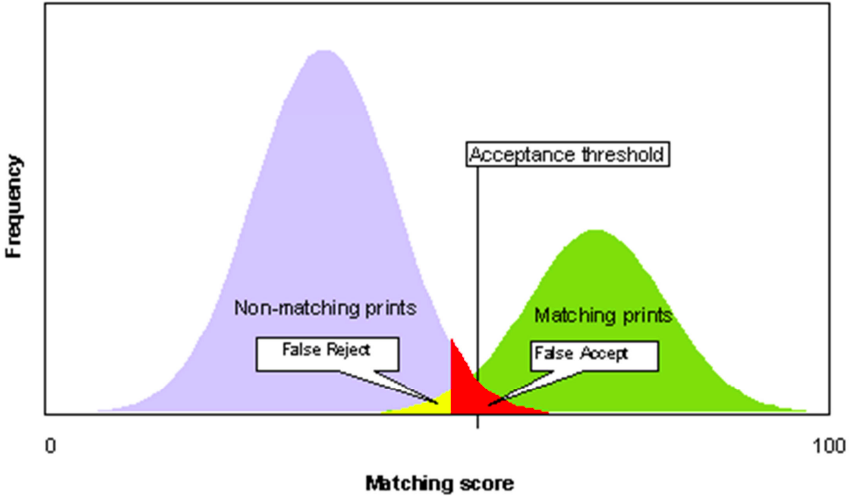
\includegraphics[width=0.5\textwidth]{/home/lorenzo/Notes/Information System Security/images/Screenshot from 2024-11-16 15-05-31.png}
        \end{minipage}
        
        \item \textbf{Psychological Acceptance:} Many people fear the "Big Brother" scenario—personal data collection and potential privacy invasions.
        \item \textbf{Irreplaceability:} Once compromised, biometric data cannot be changed, unlike a password or PIN. Thus, biometrics are primarily useful for local authentication but unsuitable for global identity systems.
        \item \textbf{Lack of Standardization:} High development costs and dependency on specific vendors are significant drawbacks in current biometric systems.
    \end{itemize}}
\end{quotebox-red}
\newpage
\section{Kerberos Authentication System}
\begin{minipage}{0.8\textwidth}
\vspace{-0.5cm}
Kerberos is a widely-used \underline{authentication protocol} based on a Trusted Third Party (TTP) model. It's designed to ensure that user passwords are never transmitted over the network. Instead, the password is used locally for encryption.
\begin{itemize}
    \item \textbf{Realm:} Refers to a Kerberos domain, grouping together all systems that use Kerberos for authentication.
    \item \textbf{Credential:} A unique identifier for a user, typically in the format \textbf{user.instance@realm}.
    \end{itemize}
\end{minipage} 
\hspace{-1.2cm}
\begin{minipage}{0.3\textwidth}
    \centering
    
\includegraphics[width=0.23\textwidth]{/home/lorenzo/Notes/Information System Security/images/Screenshot from 2024-11-16 15-19-27.png}
\end{minipage}

\subsection{Players}
There are 4 key players:
\begin{itemize}
    \item \textbf{Client (User/Application:)} the person or application trying to access a resource.
    \item \textbf{Authentication Server (AS):} Confirms who you are and issues a Ticket Granting Ticket (TGT).
    \item \textbf{Ticket Granting Server (TGS):} Issues tickets for specific services after seeing the TGT.
    \item \textbf{Service (Server):} The resource you want to access. 
\end{itemize}

\subsection{How it Works?}
\begin{figure}[h]
    \centering
    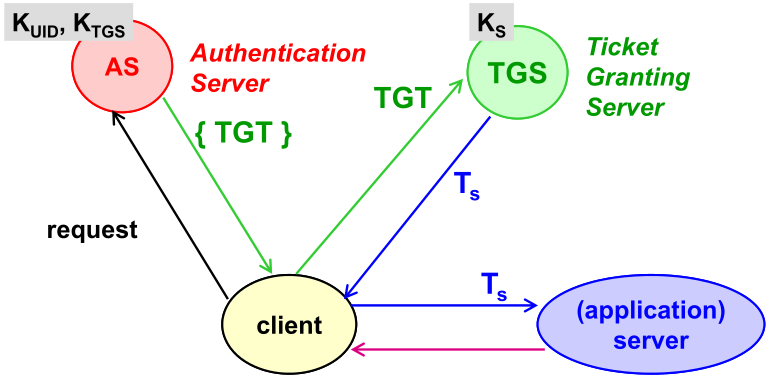
\includegraphics[width=0.5\textwidth]{/home/lorenzo/Notes/Information System Security/images/Screenshot from 2024-11-16 16-35-14.png}
\end{figure}
\begin{enumerate}
    \item \textbf{TGT Request}: Client authenticates with the Authentication Server (AS) to obtain a Ticket Granting Ticket (TGT).\vspace{0.5cm}
    \begin{minipage}{0.5\textwidth}
    %	\vspace{-0.5cm}
        \begin{customquote}
        The expression \({KC,TGS,{TC,TGS}\ KTGS}KC\) represents a \textbf{TGT}:
        \begin{itemize}
            \item The enitre structure is encrypted using the client's secret key (\(KC\)) (This ensure that only the intended client can decrupt and use the TGT).
            \item \({TC,TGS}\ KTGS\) is the \textbf{TGS} that contains the client’s identity and other information. It's encrypted using the TGS's secret key (\(KTGS\)), ensuring only TGS can read and verify the ticket. 

        \end{itemize}
        \end{customquote}
    \end{minipage} 
    \hspace{1cm}
    \begin{minipage}{0.3\textwidth}
        \centering
        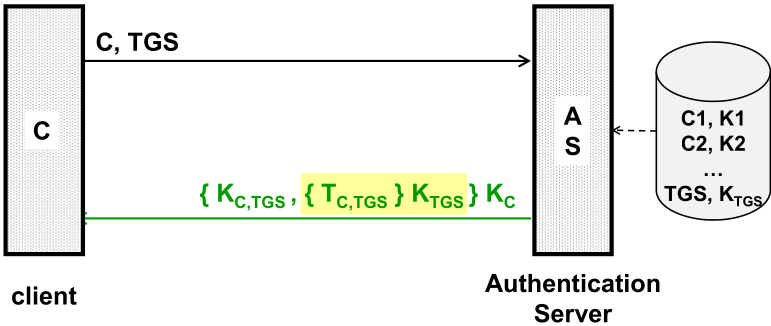
\includegraphics[width=1.3\textwidth]{/home/lorenzo/Notes/Information System Security/images/Screenshot from 2024-11-16 17-02-07.png}
    \end{minipage}

    \item \textbf{Service Ticket Request}: TGT is sent to the Ticket Granting Server (TGS) to request a service-specific ticket. \\
    \\
    \begin{minipage}{0.5\textwidth}
    %	\vspace{-0.5cm}
        \begin{customquote}
        \begin{itemize}
            \item The client sends: (S) \(\rightarrow\) the indetifier of the target device, \({TG,TGS}\ KTGS\) \(\rightarrow\) TGS ticket and \(({AC}\ KC,TGS)\) \(\rightarrow\) the authenticator.
            \item TGS Verifies and Responds: 
            \begin{itemize}
                \item The TGS decrypts the TGS ticket using its secret key (KTGS).
                \item It verifies the client's identity using the authenticator.
                \item If successful, the TGS generates a Service Ticket \(({TC,S}\ KS)\) encrypted with the secret key \((KS)\), ensuring only the service can read it; and a new session key \((KC,S)\), shared between the client and the service.
            \end{itemize}
        \end{itemize}
        \end{customquote}
    \end{minipage} 
    \hspace{1cm}
    \begin{minipage}{0.3\textwidth}
        \centering
        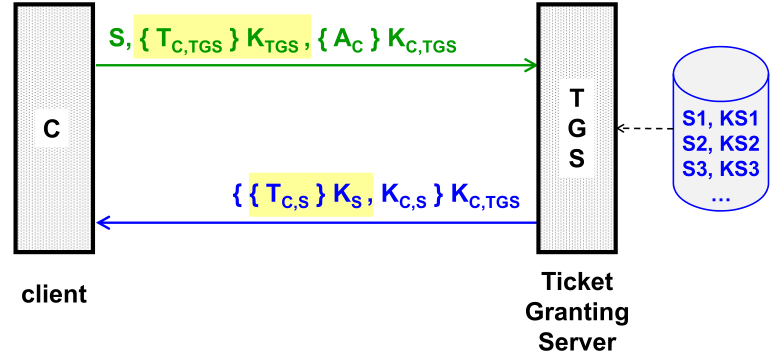
\includegraphics[width=1.4\textwidth]{/home/lorenzo/Notes/Information System Security/images/Screenshot from 2024-11-16 17-21-43.png}
    \end{minipage}
    
    \item \textbf{Access Service}: Client uses the service ticket to authenticate and access the resource. \\
    \\
    \begin{minipage}{0.5\textwidth}
        \begin{customquote}
            The client send:
            \begin{itemize}
                \item The service ticket encrypted using the service's secret key (\(KS\)), so only the service can decrypt and validate it. 
                \item The authenticator encrypted using the session key (\(KS,S\)) shared bewteen the client and the service.
        \end{itemize}
            The service responds with a response in which confirms succesfully authentication. It encrypts the message with the session key \((KC,S)\) to ensure it's secure and readable only by the client.
            
        \end{customquote}
    \end{minipage} 
    \hspace{1cm}
    \begin{minipage}{0.3\textwidth}
        \centering
        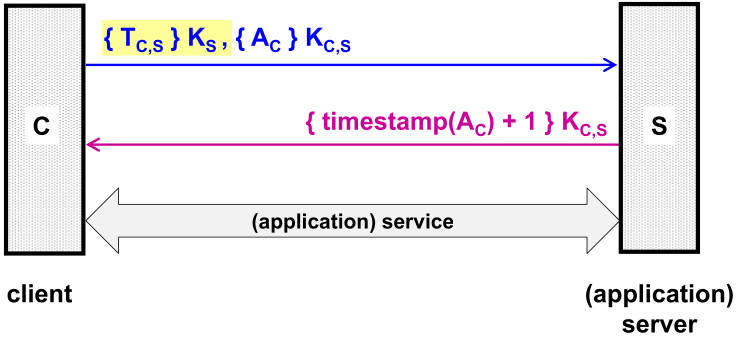
\includegraphics[width=1.4\textwidth]{/home/lorenzo/Notes/Information System Security/images/Screenshot from 2024-11-16 17-41-06.png}
    \end{minipage}
\end{enumerate}

\subsection{Single Sign-On (SSO)}
SSO allows users to authenticate once and access multiple services without repeated logins.
Types of SSO:
\begin{itemize}
    \item \textbf{Fictitious SSO:}
    \begin{itemize}
        \item Relies on tools like password synchronization or management (e.g., password wallets).
        \item Limited to specific applications.
    \end{itemize}
    \item \textbf{Integral SSO:} Uses advanced multi-application methods like Asymmetric Challenge-Response Authentication (CRA) or Kerberos.
    Often requires application changes.
    \item \textbf{Multi-Domain SSO:} Expands SSO across domains using technologies like SAML tokens, which generalize Kerberos tickets.
\end{itemize}
\textcolor{red}{\textbf{N.B.}} Single Sign-On (SSO) is not exclusive to Kerberos, but Kerberos is one of the prominent technologies that implements SSO capabilities.

\section{Authentication Interoperability}
Authentication interoperability define methods, standard, and protocol for performing authentication securely and efficiently. Let's start to analyze some framework.

\subsection{OATH}
The Open Authentication (OATH) framework provides standards for one-time password (OTP) and symmetric key management.
\begin{itemize}
    \item \textbf{HOTP:} Uses a shared secret key (K) and a counter (C) to generate an OTP.
    \\Function:
    \[ HOTP(K, C) = sel(HMAC-h(K, C))\ \&\ 0x7FFFFFFF\] 
    The result is truncated and transformed into an N-digit code (e.g., 6 digits)\footnote{K-> shared key, C -> counter, sel -> function to select 4 bytes out of a byte string}.
    
    \item \textbf{TOTP:} Similar to HOTP but uses time intervals (TS) instead of counters.\\
    Function:
    \[C = (T - T0) / TS\]\
    With default values: \(T0\) -> Unix epoch, \(TS\) -> 30-second intervals, \(T\) -> unixtime (now).
    \item \textbf{OCRA} (OATH Challenge-Response Algorithm)
    \item \textbf{PSKC} (Portable Symmetric Key Container): XML-based format for symmetric key transport.
    \item \textbf{DSKPP} (Dynamic Symmetric Key Provisioning Protocol): A client-server protocol for securely provisioning symmetric keys.
\end{itemize}

\subsection{Google Authenticator}
Supports HOTP and TOTP with adjustments for usability:
\begin{itemize}
    \item \textbf{K:} Base-32 encoded.
    \item \textbf{C:} 64-bit unsigned integer.
    \item \textbf{sel(X):} Uses the 4 least-significant bits of X to locate a portion of the result.
    \item \textbf{Defaults:} TS = 30 seconds, N = 6 digits (zero-padded if necessary).
\end{itemize}

\subsection{FIDO (Fast Identity Online)}
FIDO, developed by the FIDO Alliance, improves authentication by offering secure, password-less, and multi-factor methods. It uses biometric data locally to unlock cryptographic keys and employs asymmetric cryptography for signing challenges or transactions. FIDO prevents phishing by ensuring that authentication responses cannot be reused. Each response is a unique signature created over various data, including the Relying Party (RP) identity, making it specific to the service being accessed. Additionally, a new key pair is generated during each registration, which prevents the association of a user’s identity across different services or accounts.
\subsubsection{FIDO's frameworks include:}
\begin{itemize}
    \item \textbf{UAF} (The Universal Authentication Framework): for password-less login.
    \item \textbf{U2F} (Universal 2nd Factor) for device-based two-factor authentication.
    \item \textbf{FIDO2}: integrates U2F with WebAuthn for robust web authentication.
\end{itemize}























